% ICDM 2026 Teen Research Track.
% Requirements taken from https://icdm2026.neu.edu.cn/CallforTeen_en/list.htm :
%   * up to 5 pages INCLUDING all figures, tables and references
%   * IEEE Computer Society Proceedings Manuscript Formatting Guidelines
%   * single-blind (authors visible)
%   * first author must be a high school student, and the affiliation must say so
\documentclass[conference]{IEEEtran}
\IEEEoverridecommandlockouts

\usepackage{amsmath,amssymb}
\usepackage{booktabs}
\usepackage{graphicx}
\usepackage{xcolor}
\usepackage[colorlinks=true,linkcolor=black,citecolor=black,urlcolor=blue]{hyperref}
\usepackage{microtype}
\usepackage{balance}

\newcommand{\dR}{\Delta R}

\begin{document}

\title{Correcting Step-Cached Diffusion Transformers\\ with a Trajectory Objective}

% TODO(author): the Teen track requires a high school student as first author, and
% the affiliation must contain the words "High School Student". Fill in below.
\author{
\IEEEauthorblockN{First Author}
\IEEEauthorblockA{High School Student, \textit{School Name}\\
first.author@example.com}
\and
\IEEEauthorblockN{Second Author}
\IEEEauthorblockA{\textit{Affiliation}\\
second.author@example.com}
}

\maketitle

\begin{abstract}
Step caching accelerates diffusion transformers by reusing a block's residual
across neighbouring solver steps, which is fast but degrades the image. A learned
corrector can predict the reuse error, and the obvious way to train one is to
regress the residual it should have produced. We show that this objective is the
wrong one, and that replacing it costs twenty minutes of training.
The error a cache introduces is \emph{integrated along the sampling trajectory}
--- a refresh restores the cache, not the latent --- so a per-step residual target
is defined on a trajectory the corrector never visits. Training the same corrector
against the deviation of the latent trajectory instead, by backpropagating through
the cached rollout, improves image quality at every injection granularity we
tested ($K=1$ to $28$, all significant, $t=2.7$ to $7.0$, $n=72$).
At a fixed step count on PixArt-$\Sigma$-XL-2-512, the resulting corrector reaches
SSIM $0.6820$ against the exact output at $3.41\times$ speedup, beating a
reproduction of the TaylorSeer extrapolation mechanism by $+0.0946$ SSIM
(\mbox{$t=14.5$}, improving on all $72$ of $72$ paired cases) for $8.4\%$ less
speedup, and a reproduction of the Block Caching mechanism by $+0.0490$
($t=8.4$) while being $12\%$ faster than it. We also report the measurement that
motivated the change: driving residual accuracy $25$--$43\%$ better by matched-data
retraining buys only $+0.005$ to $+0.013$ SSIM, so residual error is a poor guide
to what a corrector is worth.
\end{abstract}

\begin{IEEEkeywords}
diffusion models, inference acceleration, feature caching, diffusion transformers
\end{IEEEkeywords}

\section{Introduction}

Sampling from a diffusion transformer costs one full forward pass per solver step.
Step caching exploits the fact that consecutive steps produce similar internal
features: at an \emph{anchor} step the residual $R=\mathrm{block}(h)-h$ of each
transformer block is computed and stored, and for the next $i-1$ \emph{reuse} steps
the block is skipped and its stored residual added instead
\cite{ma2024deepcache,selvaraju2024fora,chen2024deltadit}. This is cheap and
training-free, and it visibly degrades the image.

Two families of fixes exist. Training-free extrapolation predicts the residual's
drift from its own history \cite{liu2024teacache,liu2025taylorseer}, and learned
correction trains a small network to predict the reuse error
\cite{wimbauer2024blockcaching,ma2024l2c}
\begin{equation}
\dR \;=\; R_{\text{true}} - R_{\text{anchor}},
\label{eq:target}
\end{equation}
which is exactly the error verbatim reuse commits. Learned correction is the
setting of this paper. Its natural training objective is supervised regression on
\eqref{eq:target}, and every design decision then follows from residual accuracy:
architecture, checkpoint selection, and how much correction to inject.

Our contribution is that this objective is misaligned, and that the misalignment is
both diagnosable and cheap to fix.

\begin{enumerate}
\item We measure the deviation of the cached trajectory from the exact one at every
solver step, and find that it does \emph{not} reset at cache refreshes: it climbs
almost monotonically ($0.0089$ at step 1 to $0.6092$ at step 19). An anchor refreshes
the cache, not the latent, so deviation already injected into the state is permanent.
Residual error is pointwise; trajectory error integrates.
\item We show that pushing residual accuracy hard does not pay. Matching training
data volume across granularities and training every rung to convergence improves
residual error by $25$--$43\%$ and image SSIM by only $+0.005$ to $+0.013$,
against $+0.033$ for the decision to add correction at all.
\item We train the same corrector against the trajectory deviation instead, by
backpropagating through the cached rollout. This is inexpensive for a reason
specific to caching: a cached block never executes, so the graph over one reuse
step is $K$ corrector forwards rather than $K$ transformer blocks. It improves
image quality at every $K$, and by the largest margin where per-site correction
degrades worst.
\item At a fixed step count it beats reproductions of two published mechanisms on
three fidelity metrics, at a speedup cost of $8.4\%$ against one of them and a
speedup \emph{advantage} against the other.
\end{enumerate}

\section{Related Work}

\paragraph*{Fewer steps versus cheaper steps}
Two orthogonal routes reduce sampling cost. Distillation and consistency training cut
the number of steps \cite{salimans2022progressive,song2023consistency}, and
high-order solvers do the same without retraining \cite{lu2022dpmsolver}. Caching
instead makes each step cheaper, so the two compose. We hold the step count and the
solver fixed throughout, which isolates the caching question but also means our
comparisons say nothing about which route is preferable --- see Limitations.

\paragraph*{What to cache}
Feature caching for diffusion U-Nets \cite{ma2024deepcache} carries over to
transformers, where the natural unit is a block's residual
\cite{selvaraju2024fora,chen2024deltadit}, optionally chosen adaptively per step
\cite{liu2024teacache} or per token \cite{zou2024toca}. All of these decide
\emph{when} to skip; we take the schedule as given and ask what to add back.

\paragraph*{Correcting a cached step}
Block Caching \cite{wimbauer2024blockcaching} applies a timestep-conditioned
per-channel scale-shift to the reused feature --- trained, but a function of the
timestep alone. TaylorSeer \cite{liu2025taylorseer} forecasts the residual from its
own history by finite differences, requiring no training. Learning to cache
\cite{ma2024l2c} learns the skip pattern rather than a correction. Our corrector
differs from all three in reading the \emph{current state}, which is what makes
error propagation across injection sites multiplicative
(Sec.~\ref{sec:granularity}) and is also why the choice of training objective
matters at all: a state-independent correction cannot be improved by observing the
trajectory it produces.

\paragraph*{Objectives defined on a policy's own trajectory}
Regressing a target collected off-policy and deploying it in closed loop is the
setting DAgger addresses in imitation learning \cite{ross2011dagger}, and scheduled
sampling addresses in sequence models \cite{bengio2015scheduled}. Both fix the data
distribution. Our finding is that in this setting the data distribution is not the
binding problem --- the objective is --- and that because the cached rollout is
differentiable, the trajectory can be optimised directly rather than approached by
resampling.

\section{Setup}

\paragraph*{Backbone and schedule}
PixArt-$\Sigma$-XL-2-512 \cite{chen2024pixartsigma} (0.6B parameters, 28 blocks) with
its shipped DPM-Solver++ scheduler \cite{lu2022dpmsolver} at 20 steps and $512^2$
resolution. Anchors are uniform at interval $i=5$, so 4 anchor steps and 16 reuse
steps. All numbers are against the same-seed exact 20-step output.

\paragraph*{Corrector}
A conditioned MLP (11.9M parameters) reads the state drift $h_t-h_{\text{anchor}}$,
the cached residual, and the anchor hidden state, conditioned on the diffusion
timestep, the reuse horizon $\tau$, and the site index. At deployment
\begin{equation}
h_{\text{out}} \;=\; h_t + R_{\text{anchor}} + \sigma\,\widehat{\dR},
\label{eq:deploy}
\end{equation}
where $\sigma$ is an injection strength selected on validation and never on test.
The state-drift input is what makes the correction state-dependent, which matters
in Sec.~\ref{sec:granularity}. The 28 blocks are grouped into $K$ contiguous cached
segments, so $K$ is the number of injection sites per reuse step; $K=1$ corrects the
whole stack once and $K=28$ corrects every block.

\paragraph*{Protocol}
Every image-level number is a paired comparison over 24 held-out prompts $\times$ 3
seeds ($n=72$), with $\sigma$ re-selected on validation for each corrector over a
common grid. We report $t$ statistics and the number of cases that improve.
Prompts are templated (10 styles $\times$ 24 subjects $\times$ 10 conditions); the
held-out split shares no subject with training.

\section{Residual accuracy is a poor guide}
\label{sec:diagnosis}

\paragraph*{Trajectory error integrates}
Measuring $\|x_{\text{cached}}-x_{\text{exact}}\|/\|x_{\text{exact}}\|$ at each of
the 20 steps shows deviation rising from $0.0089$ to $0.6092$ with only small dips
at the four anchors. This is the basic reason a per-step residual target is
misaligned: the corrector's action at step $t$ changes the state at $t+1$, while
\eqref{eq:target} is defined on the unperturbed trajectory.

\paragraph*{Better residual accuracy barely helps}
To rule out the possibility that the residual objective simply had not been
optimised hard enough, we rebuilt training from scratch: data volume matched across
granularities at exactly 50{,}176 slots per rung (a seed multiplier of $28/K$), and
the step budget selected per rung on validation by doubling until the gain fell
below $0.5\%$. Residual error improved by $25$--$43\%$ depending on $K$. Image SSIM
improved by $+0.0131$ at $K=1$ falling to $+0.0055$ at $K=7$ --- all significant,
all small. Two trends run opposite along the granularity axis: the achievable
residual improvement rises with $K$ ($-27.7\%$ at $K=1$ to $-42.9\%$ at $K=28$)
while the image quality it buys falls.

\paragraph*{A ceiling check}
Replacing the corrector by an oracle that recovers a fraction $\beta$ of the true
residual gives residual error exactly $(1-\beta)^2$, so each trained corrector has an
equivalent $\beta$. Final-step trajectory error falls from $0.6102$ at $\beta=0$ to
$0.4384$ at $\beta=0.8$, and to exactly $0$ at $\beta=1$. The curve is convex: the
ceiling is perfect and the middle is flat, which rules out the correction
form as the limit and locates the problem in the objective. Notably the trained
correctors beat an oracle at their own equivalent $\beta$ by about $1.5\times$,
because a scalar oracle shrinks error isotropically while a trained corrector learns
which directions matter to the trajectory. Residual error therefore distorts in both
directions: as an objective it overstates the gain, as a capability measure it
understates the corrector.

\section{Training against the trajectory}

We keep the architecture, the schedule and the deployment rule \eqref{eq:deploy},
and change only the loss. Let $x_1,\dots,x_T$ be the cached latents and
$x^\star_1,\dots,x^\star_T$ the exact ones under the same seed. The objective is
\begin{equation}
\mathcal{L} \;=\; \sum_{t \in \text{reuse}}
\frac{\|x_t - x^\star_t\|^2}{\|x^\star_t\|^2},
\label{eq:loss}
\end{equation}
minimised by backpropagating through the cached rollout. Supervision is free: the
exact trajectory comes from the same forward pass that produces the corrector's
input, so no annotation is involved.

Two implementation facts make this practical, and both are specific to caching.
First, a cached block never runs its transformer block --- the runtime returns
$h_t + R_{\text{anchor}} + \sigma\widehat{\dR}$ --- so the graph over one reuse step
consists of $K$ corrector forwards, not $K$ blocks of a 0.6B model. Peak memory is
$7.5$\,GB at $K=1$; checkpointing each corrector call brings $K=14$ from over
$44$\,GB down to $4.2$\,GB. Second, gradients are cut at anchor steps, where the cache
is refreshed from exact values, so a corrector call can only influence later
intervals through the latent. Extending the graph across intervals improves
\eqref{eq:loss} but does not improve image metrics, so we keep the one-interval
truncation. Training is 400 steps, about 20 minutes on one A40.

\section{Results}

\subsection{Fixed step count against published mechanisms}

Table~\ref{tab:main} compares at 20 steps and $i=5$, so every arm skips the same
blocks and speedup differs only by each method's correction overhead. We reproduce
the TaylorSeer mechanism \cite{liu2025taylorseer} (Newton divided-difference
forecast of the residual from its history, training-free) and the Block Caching
mechanism \cite{wimbauer2024blockcaching} (a timestep-conditioned per-channel
scale-shift, trained but state-independent). Both are reimplemented in our runtime
rather than run from the authors' code, so they are reproductions of the mechanisms
under our schedule and backbone, not replications of the published results.

\begin{table}[t]
\centering
\caption{Fixed 20 steps, $i=5$, $n=72$. ``Sp.'' is measured wall-clock speedup
against the exact model; $\Delta$SSIM is paired against verbatim caching. The two
reproduced mechanisms are described in the text.}
\label{tab:main}
\small
\begin{tabular}{@{}lccccc@{}}
\toprule
Method & Sp.\ & SSIM$\uparrow$ & PSNR$\uparrow$ & LPIPS$\downarrow$ & $\Delta$SSIM \\
\midrule
Exact, 20 steps   & 1.72 & 0.7951 & 21.78 & 0.1786 & --- \\
Verbatim cache    & \textbf{3.79} & 0.6269 & 15.37 & 0.4669 & --- \\
TaylorSeer, 1st   & 3.72 & 0.5874 & 14.31 & 0.5080 & $-0.0395$ \\
TaylorSeer, 2nd   & 3.73 & 0.4782 & 13.57 & 0.6386 & $-0.1487$ \\
Block Caching     & 3.04 & 0.6330 & 15.66 & 0.4594 & $+0.0060$ \\
Residual obj.     & 3.41 & 0.6676 & 16.48 & \textbf{0.3795} & $+0.0407$ \\
\textbf{Trajectory obj.} & 3.41 & \textbf{0.6820} & \textbf{17.20} & 0.3883 & $\mathbf{+0.0551}$ \\
\bottomrule
\end{tabular}
\end{table}

Paired against the trajectory-objective corrector, the first-order TaylorSeer
mechanism loses $0.0946$ SSIM ($t=14.5$) and $0.1197$ LPIPS ($t=14.2$), with our
corrector better on all 72 of 72 cases; the second-order version loses $0.2038$
($t=39.8$, 72/72); Block Caching loses $0.0490$ ($t=8.4$, 64/72). The exchange rate
is therefore favourable: $8.4\%$ less speedup than TaylorSeer for $+0.0946$ SSIM,
and against Block Caching we are both faster and better.

Two qualifications belong with the table. TaylorSeer at $i=5$ is \emph{worse than no
correction at all} ($-0.0395$, only 3 of 72 cases improve); in our reproduction it
helps at $i=2$--$3$ and is past its useful extrapolation range by $i=5$, so
Table~\ref{tab:main} is not evidence against it at its own operating point. And
TaylorSeer is training-free, while our corrector costs training time, 11.9M
parameters and $0.041$\,TFLOP per correction --- which is exactly where the $8.4\%$
goes.

\subsection{The objective change helps at every granularity}
\label{sec:granularity}

\begin{figure}[t]
\centering
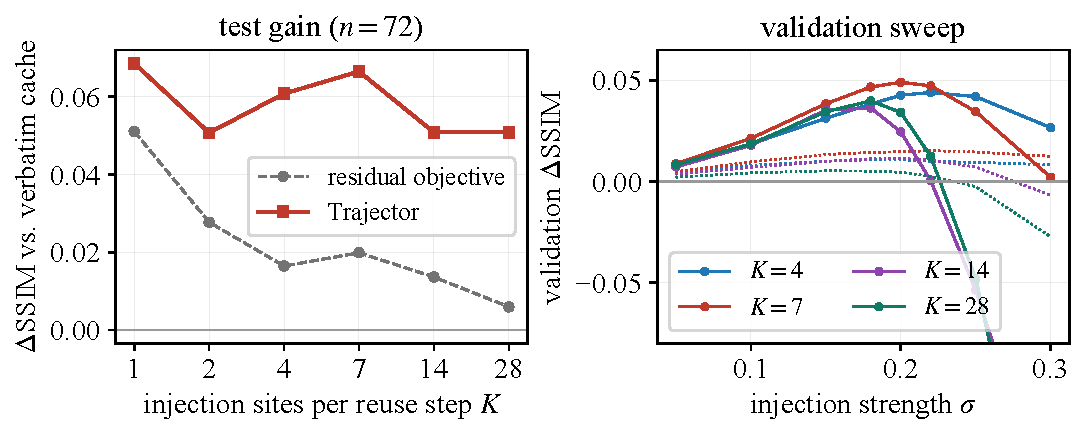
\includegraphics[width=\columnwidth]{figs/icdm_main.pdf}
\caption{Left: gain over verbatim caching at each granularity under the two
objectives, each at its own validation-selected $\sigma$. Right: sensitivity to
$\sigma$ for the high-$K$ correctors; the optimum moves left and the peak narrows
as $K$ grows, and $K\!=\!14$ and $K\!=\!28$ turn negative by $\sigma=0.25$.}
\label{fig:main}
\end{figure}

\begin{table}[t]
\centering
\caption{Per-granularity comparison of the two objectives, $n=72$, each at its own
validation-selected $\sigma$.}
\label{tab:perk}
\small
\begin{tabular}{lccc}
\toprule
$K$ & Residual obj. & Trajectory obj. & Difference \\
\midrule
1  & $+0.0406$ & $+0.0553$ ($\sigma\!=\!0.60$) & $+0.0147$ ($t=2.7$) \\
2  & $+0.0149$ & $+0.0385$ ($\sigma\!=\!0.30$) & $+0.0236$ ($t=3.8$) \\
4  & $+0.0189$ & $+0.0450$ ($\sigma\!=\!0.22$) & $+0.0261$ ($t=5.0$) \\
7  & $+0.0145$ & $\mathbf{+0.0515}$ ($\sigma\!=\!0.18$) & $\mathbf{+0.0370}$ ($t=7.0$) \\
14 & $+0.0096$ & $+0.0414$ ($\sigma\!=\!0.18$) & $+0.0318$ ($t=4.7$) \\
28 & $+0.0148$ & $+0.0380$ ($\sigma\!=\!0.18$) & $+0.0232$ ($t=4.8$) \\
\bottomrule
\end{tabular}
\end{table}

Table~\ref{tab:perk} and Fig.~\ref{fig:main} show the objective change helping at
all six granularities, every difference significant. The margin is largest where
per-site correction degrades worst: $+0.0370$ at $K=7$ against $+0.0147$ at $K=1$.
This is consistent with the mechanism behind the degradation. A state-dependent
correction turns error propagation across sites multiplicative rather than additive
--- $\delta_{b+1}\approx(I+J_b)\delta_b+\epsilon$ with $J_b=\partial\widehat{\dR}/\partial h$
--- and the trajectory objective is the only one that observes the consequence of
that compounding rather than pointwise error. The degradation is weakened, not
removed: the residual objective's gain falls $3$--$4\times$ from $K=1$ to high $K$
while the trajectory objective's falls $1.2$--$1.8\times$.

Fig.~\ref{fig:main} (right) also shows why $\sigma$ must be re-selected per
corrector. The optimum moves from $0.60$ at $K=1$ to $0.18$ at high $K$, and the
peak narrows sharply: $K=4$ stays above $+0.039$ across $\sigma\in[0.18,0.25]$ while
$K=14$ and $K=28$ are already negative at $\sigma=0.25$. Both corrector generations
trace the same family of curves, so this is a property of granularity rather than of
the objective.

\begin{figure}[t]
\centering
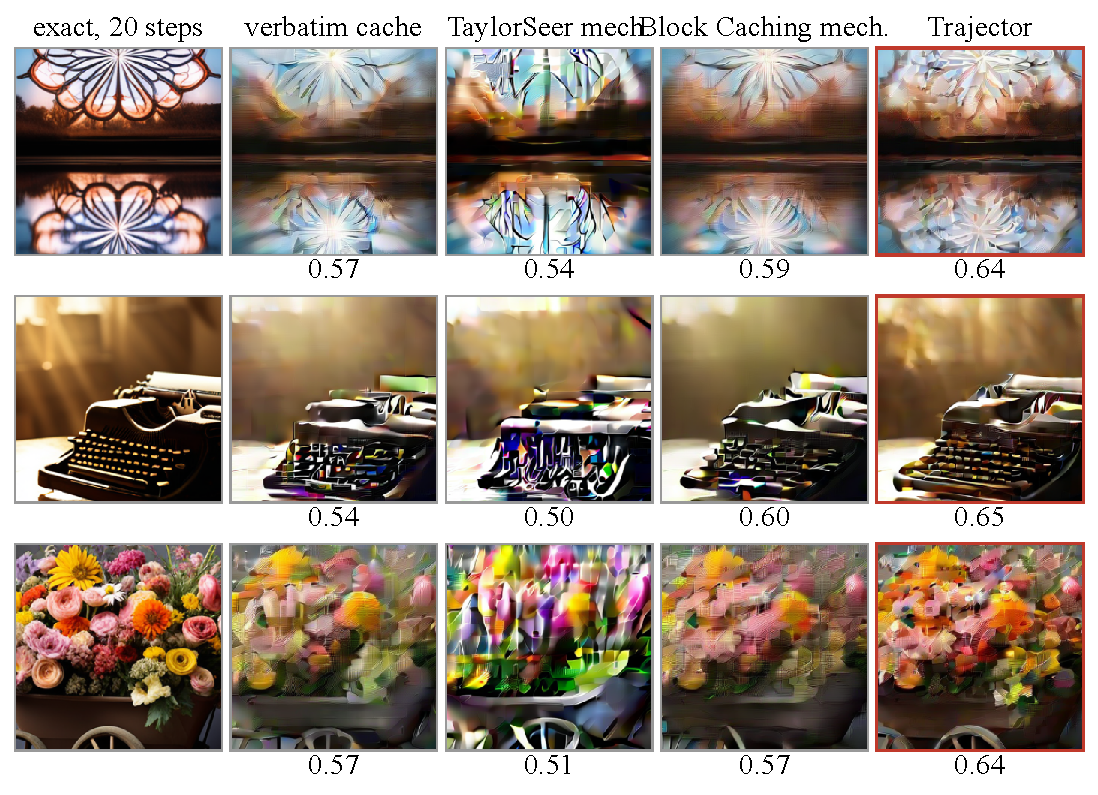
\includegraphics[width=\columnwidth]{figs/icdm_qual.pdf}
\caption{Native-resolution $250^2$ crops, same seed and prompt across a row, SSIM
against the exact output below each panel. Crops rather than downscaled images
because thumbnails hide the texture differences these methods differ in.}
\label{fig:qual}
\end{figure}

Fig.~\ref{fig:qual} shows the same three prompts under each method, and the failure
modes differ in kind rather than in degree. Verbatim caching smears surface detail
into streaks and flattens the background gradient. The TaylorSeer mechanism's
dominant artefact is not lost detail but \emph{colour} --- extrapolating the residual
introduces chromatic fringing along edges, which is consistent with it scoring worst
on LPIPS in Table~\ref{tab:main} despite skipping the same blocks. The Block Caching
mechanism keeps structure cleaner but renders tone flatter and leaves local bloom
artefacts, which its per-channel scale-shift can shift but not localise. Our
correction recovers the background gradient most closely and leaves the least
fringing, though not none.

\section{Limitations}

\paragraph*{One backbone, and it saturates early}
Measuring the exact model against step count reveals that ImageReward
\cite{xu2023imagereward} is saturated by 10 steps on this backbone (102\% of a
100-step reference) while pixel fidelity keeps improving. Any method selling saved
compute therefore competes against an already-saturated baseline here, and an
equal-compute comparison on this backbone favours simply lowering the step count.
That is a property of PixArt-$\Sigma$ with a high-order solver, not a verdict on
caching, which is why we compare at fixed step count. Whether our results transfer
to a backbone that needs many steps is untested.

\paragraph*{Metrics disagree}
We report SSIM, PSNR and LPIPS because no single one is decisive. An objective
trained on LPIPS wins on LPIPS ($+0.1067$ over verbatim caching) and loses on SSIM
and PSNR; ImageReward cannot separate the objectives at all ($t=0.2$ to $1.2$),
though it does separate every corrector from verbatim caching ($+0.33$ to $+0.40$,
all $t>4$). Which reward to prefer is not answerable from our evidence.

\paragraph*{Scope}
Templated prompts (24 training subjects), $512^2$ only, 24 held-out prompts $\times$
3 seeds, and a corrector trained for 400 steps without hyperparameter search from a
residual-trained initialisation --- so the reported gain is marginal over that
initialisation rather than a standalone method. Correctors trained to low residual
error can overflow fp16 at deployment; we deploy the high-$K$ ones in fp32.

\section{Conclusion}

The natural objective for a learned cache corrector --- regress the residual it
should have produced --- is misaligned with what caching actually damages, because
cache error integrates along the sampling trajectory while residual error is
pointwise. Optimising the residual objective harder is a poor investment: a
$25$--$43\%$ residual improvement buys $+0.005$ to $+0.013$ SSIM. Replacing the
objective with the trajectory deviation, which costs 20 minutes of training and no
architectural change, improves image quality at every injection granularity we
tested, and at a fixed step count beats reproductions of two published mechanisms on
three fidelity metrics.

\section*{Reproducibility}

Code, configurations, per-run logs and the raw per-case metrics behind every number
are available at \url{https://github.com/xiaruize0911/Diff-cache-Comp}. Feature
collection is seeded and reproducible bit-for-bit; every table cell can be recomputed
from the archived \texttt{results.json} files.

\balance
\bibliographystyle{IEEEtran}
\bibliography{refs}

\end{document}
